%%%%%%%%%%%%%%%%%%%%%%%%%%%%%%%%%%%%%%%%%%%%%%%%%%%%%%%%%%%%%%%%%%%%%%%%%%%%%%%%%%%%%%%%%%%%%%%%%%%%
%
% NOTE TO AIP TYPSETERS: TO CONVERT FROM TWO-COL TO PREPRINT, SWITCH
% COMMENTOUT COMMAND FROM A TO B IE. use
% \newcommand{\commentoutA}[1]{}
% \newcommand{\commentoutB}[1]{#1}
% instead of the following
\newcommand{\commentoutA}[1]{#1}
\newcommand{\commentoutB}[1]{}
\renewcommand{\thefootnote}{\fnsymbol{footnote}}

%,twocolumngrid%
%,secnumarabic%

%\documentclass[prl,twocolumngrid,twocol,secnumarabic,amssymb]{revtex4}


\commentoutA{\documentclass[prb,aps,twocolumn,twocolumngrid,secnumarabic,superbib,hyperref]{revtex4}}
\commentoutB{\documentclass[aps,nobibnotes,superbib,byrevtex,preprint]{revtex4}}
\usepackage{graphicx}
\usepackage{amsfonts}
\usepackage{amsmath}
\usepackage{bm}
\usepackage{alltt}
%\usepackage{epsfig}
%%
%%

\begin{document}

\date{\today}

\title{Trace setting density matrix purification in first-principles
linear scaling electronic structure calculations}

\author{Anders~M.~N.~Niklasson\cite{Corr}}
\author{C.~J.~Tymczak}
\author{Matt Challacombe\homepage{www.t12.lanl.gov/~mchalla}}
\affiliation{
Theoretical Division, Los Alamos National Laboratory,
Los Alamos, NM 87545, USA}

\begin{abstract}
A scheme for the construction of the density matrix in terms of
a purification expansion of the Hamiltonian operator is proposed. The scheme
works with a predefined occupation number and does not need
the additional adjustment or prior knowledge of the chemical potential.
In this sense the method is related to the trace preserving canonical 
purification scheme by Palser and Manolopoulos \cite{McWeeny60,Palser98}, 
but instead of a fixed trace criteria we only require the correct
occupation at convergence. The two methods are
compared within the MondoSCF suite of linear scaling self-consistent total energy
programs \cite{Mondo} for different materials, and we find an overall 
improved performance, especially at low and high occupancies. In comparison
with some variational methods the two schemes has the major advantage of
dealing also with degenerate eigenstates and fractional occupancy. 
Formulas for calculating the fractional filling and degeneracy from 
the density matrix are derived, and alternative critereas to idempotency
in the case of degeneracy and fractional filling are suggested.
Thresholding is analyzed regarding numerical stability and error.
Quadratic convergence in total energy as a function of thresholding
is demonstrated.
%
%\keywords{density matrix, purification, linear scaling, electronic structure,
%spectral projection, degeneracy}
%
\end{abstract}

\maketitle

\section{Introduction}

For non-metallic systems it is now possible to solve the Self-Consistent-Field 
equations for systems with thousands of atoms using linear scaling methods. These methods 
achieve a reduced ${\cal O}(N)$ computational complexity, where $N$ is the number of basis 
functions assumed proportional to system size. In contrast, conventional formulations of 
Self-Consistent-Field theory such as the Roothaan-Hall\cite{CRoothaan51} and Kohn-Sham\cite{Kohn65} 
method involve an ${\cal O}(N^3)$ solution to an eigenvalue problem 
\begin{equation}\label{EgenvalueProblem}
\bf F C = \bf e \bf C.
\end{equation}
Here $\bf F$ is the Fockian, the effective single-particle Hamiltonian 
in an orthogonal representation. The notation in this paper follows the Roothaan-Hall 
method, but is traighforward to apply also to the Kohn-Sham scheme in density functional theory.
The matrix $\bf C$ is spanned by eigenvectors (molecular orbitals), ${\bf c}_k$, which may be 
used to construct the first order reduced density matrix via the outer product
\begin{equation}\label{Density}
{\bf P} = \sum_{k=1}^{N_{\rm el}} {\bf c}^{\rm T}_{k} {\bf c}_{k},
\end{equation}
while the vector $\bf e$ is spanned by the eigenvalues $e_i$ that determine 
the electronic single-particle energy
\begin{subequations}
\begin{eqnarray} 
E_{\rm el} &=& \sum_{i=1}^{N_{\rm el}} e_i \label{EigenEnergy}  \\
&=&{\rm Tr}[ \bf P F ], \label{TraceEnergy} 
\end{eqnarray}
\end{subequations}
with $N_{\rm el}$ the number of occupied states.

Many of these linear scaling methods involve iteratively constructing the density matrix 
in a local, non-orthogonal basis, exploiting the approximately exponential decay of matrix
elements with basis function seperation through the use of  sparse matrix technologies.  
These technologies include linear algebra kernals such as the sparse matrix-matrix multiplication
and incomplete methods for computing congruence transformations between orthogonal and 
non-orthogonal representations.  

One approach to constructing the density matrix is via constrained functional minimization of the energy trace 
expresion, Eq.(\ref{TraceEnergy}), with $\bf P$ driven towards idempotence and electron conservation
\cite{Sameh82,Li93,Carlsson95,Hernandez96,Kohn96,Daniels97,Yang97,Stephan98,Challacombe99,Haynes99,Bowler99,Daniels99}.
This is the density matrix minimization (DMM) or the constrained functional minimization 
approach. A second approach is via polynomial approximation of
\begin{equation}
\label{Heavyside}
\bf P = \theta ( \mu \bf I - \bf F ),
\end{equation}
where $\theta$ is the Heavyside step function setting all eigenvalues
above the chemical potential $\mu$ to $0$ and all the occupied eigenvalues below $\mu$ to $1$,
forming an idempotent density matrix 
\cite{Bowler99,Daniels99,McWeeny60,Goedecker94,Palser98,Challacombe99,Beylkin99,Holas01,Niklasson02,Kenney95}.
This is the polynmial expansion (PE) or the spectral projection approach.
Both the constrained functional minimization and the spectral projection methods 
can be posed as a general expansion of the density matrix in terms of 
the Fockian, {\em i.e.} $\bf P = {\cal P}(F)$ for some polynomial ${\cal P}$.
In an iterative approach this expansion can be formulated as
\begin{subequations}
\begin{eqnarray}
&& {\bf X}_0 = {\cal P}_{0}(\bf F) \\
&& {\bf X}_{n+1} = {\cal P}_{n+1}({\bf F}, {\bf X}_n) ~~ {\rm (DMM)} \label{DMMPoly}\\
&& {\bf X}_{n+1} = {\cal P}_{n+1}({\bf X}_n)~~~~~~~~ {\rm  (PE)} \label{PEPoly}\\
&& {\bf P} = \lim_{n \rightarrow \infty} {\bf X}_n.
\end{eqnarray}
\end{subequations}



There is a subtle distinction between polynomial expansion (PE) and density 
matrix minimization (DMM) resulting due to the use of approximate sparse matrix algebra, wherein
sparsity is enforced through a radial cutoff or numerical threshold  to 
achieve $N$-scaling of the sparse matrix-matrix multiply. In polynomial expansion schemes, 
such as Chebyshev expansion and density matrix purification, 
this approximate sparse-matrix algebra leads to an {\em accumulated error} in the density matrix 
that is seperate and additional to the {\em truncation errror}.  Truncation errors are simply 
the errors that result from dropping elements of the exact density matrix.  Density matrix 
minimization methods such as the Li-Nunes-Vanderbilt\cite{xli93} (LNV) approach are able to 
avoid accumulation errors through continued use of gradient expressions that contain the Fockian, 
as implied by Eq.~(\ref{DMMPoly}). On the other hand, polynomial expansion methods lose contact 
with the Fockian after the first iteration, allowing repeated iterations with 
approximate sparse matrix algebra to blur the eigenbasis.  However, density matrix purification 
methods tend to be more efficient than density matrix minimization methods, requiring fewer 
matrix-multiplies and converging quadratically as they reach idempotence.

There are a number density matrix purification schemes worth differentiating: 
{\it 1)} {\it grand canonical} schemes, with a step function  expansion around a predefined 
         chemical potential \cite{McWeeny60,Palser98,Holas01},
{\it 2)} {\it canonical trace conserving} schemes, with a fixed trace
         in each iteration step \cite{Palser98}, 
{\it 3)} {\it trace correcting} methods, where the trace only reaches the correct value at 
         convergence \cite{Niklasson02b}, and finally 
{\it 4)} {\it trace setting} algorithms (this article), where the 
         trace is set to the correct value in most steps and towards convergence.
There are also various hybrid approaches that mix both density matrix minimization and 
purification together.  For example
Challacombe\cite{Challacombe99} used a commuting constrained minimization scheme to precondition 
a grand canonical purification scheme,
while Bowler \cite{Bowler99} suggests the use of the LNV density matrix minimization 
after purification to reduce accumulation errors.

Perhaps most closely related to the present work, a canonical trace 
conserving purification scheme, was recently constructed by Palser and Manolopoulos 
(PM) in Ref.~\onlinecite{Palser98}. 
By using a starting guess ${\bf X}_0$ with the trace equal to 
the occupation number and thereafter performing trace-conserving
spectral projections, ${\bf X}_n$ converges to the correct density matrix without
prior knowledge of the chemical potential. 

The PM scheme has an excellent
performance compared to other methods \cite{Palser98,Daniels99}, and is also
able to deal with degenerate eigensystems.  However, it has been found
to fail for certain systems such as C60 \cite{Daniels99} (MATT-Check reference!), and the accumulation
errors are to large in some cases for performing ab initio MD \cite{DBowler00} (MATT-Check reference!).
Also, due to the constraint of trace conservation the method is inefficient at low 
and high filling, $f_{occ}=N_e/N$, due to the unfavorable behavior of ${\cal P}_{\rm PM}$ near 
its endpoints.  Low filling $f_{occ}\lesssim .2$  is encounted 
with a large basis set, while high filling $f_{occ} \gtrsim .8$ corresponds to a small basis set.

In this paper, we introduce a new fourth order trace setting purification scheme (TS4) 
that is efficient also for high and low fillings.  This new method is 
efficient because it employs a polynomial that is uniformly well behaved, but with the
potential for violating trace conservation in intermediate steps.  The method
converges more rapidly for both small and large basis sets, significantly reducing 
threshold induced blurring of the eigenbasis in these cases.

The outline of this paper follows:  In Section \ref{TSP}, we define trace setting purification,
and present a fourth order algorithm.  Then, in Section \ref{Degen} we discuss the ability of
trace setting methods to cope with degenerate eigensystems.  In Section \ref{Error}, we
analyse the asymptotic behavior of both the initial accumulated error and the accumulated
error at idempotence due to thresholding. Finally, the new trace setting algorithm is compared 
to the PM scheme and the exact eigensolution on the basis of accuracy and time to convergence.

\section{Purification schemes}\label{TSP}

The general idea behind purification (spectral projection) for construction 
of the density matrix is based on an iterative expansion of the
Fockian in terms of a continuously increasing 
polynomial ${\cal P}(x)$, $x \in [0,1]$  with stationary fixed end points extremums 
at $0$ and $1$, i.e. ${\cal P}(0) = 0$, ${\cal P}(1) = 1$, and ${\cal P}'(0)={\cal P}'(1)=0$. 
It can be shown that a nested sequence of such polynomials 
converges to a step function with a step somewhere in $[0,1]$. 
First we discuss the grand canonical McWeeny method and the canonical
purification scheme before presenting the main ideas of our
trace setting purification technique.

\subsection{McWeeny purification}

The grand canonical McWeeny purification scheme \cite{McWeeny60,Palser98}
is a polynomial expansion based on the following iteration:
\begin{equation} \label{P3}
{\bf X}_{n+1} = {\cal P}_{\rm McW}({\bf X}_n) = 3 {\bf X}_n^2 - 2 {\bf X}_n^3, ~~~~~ n = 0,1,2, \ldots
\end{equation}
using the initial guess 
\begin{equation} \label{Pur2}
{\bf X}_0 = \alpha(\mu { \bf I} - {\bf F}) + \beta{ \bf I}
\end{equation}
where
\begin{equation} \label{StartG}
\alpha = {\rm min} \left\{ \beta[\varepsilon_{\rm max} - \mu]^{-1},
(1-\beta)[\mu - \varepsilon_{\rm min}]^{-1} \right\}.
\end{equation}
The constant $\beta \in [0,1]$ is the inflection point where ${\cal P}(x) = x$ and for 
the symmetric McWeeny polynomials $\beta = 1/2$. With this fixed
inflection point the step is formed at $x=0.5$. This scheme is very
efficient if the chemical potential $\mu$ is known in advance. 
Alternatively, it is possible to form a good guess through use of a commuting 
density matrix minimization as suggested in \onlinecite{MChallacombe00}, 
or $\mu$ can be adjusted until the correct trace (occupancy or population) is reached. 

\subsection{Canonical purification}

Another approach that avoids the problem with the unknown chemical
potential is to incorporate $\mu$ into the
polynomial expansion through trace conservation. This is the basis 
of the Palser-Manolopoulos\cite{Palser98} (PM) method.
The PM method starts with the correctly normalized guess ${\bf X}_0$ in Eq.\ (\ref{Pur2}) with 
the trace equal to the occupation number $N_{\rm el}$, where
\begin{equation} \left\{
\begin{array}{ll}
\alpha & = \frac{1}{N} \min \left( \frac{N_{\rm el}}{\varepsilon_{\rm max} - \mu},  \frac{N-N_{\rm el}}{\mu-\varepsilon_{\rm min}} \right), \\
\beta &\equiv f_{\rm occ}  = N_{\rm el}/N \\
\mu  &= {\rm Tr}[{\bf F}]/N.
\end{array} \right.
\end{equation}
and thereafter trace-conserving purification is performed with
\begin{equation} 
{\bf X}_{n+1}  = \left\{ 
\begin{array}{l}
[(1+c_n){\bf X}^2_n - {\bf X}^3_n]/c_n,~~ c_n \geq 1/2  \\
\left. [(1-2c_n){\bf X}_n + (1+c_n){\bf X}^2_n - {\bf X}^3_n]/(1-c_n) \right.
\end{array} \right.
\end{equation}
where
\begin{equation}
c_n  = \frac{ {\rm Tr}[{\bf X}^2_n-{\bf X}^3_n] } { {\rm Tr}[{\bf X}_n-{\bf X}^2_n] }.
\end{equation} 
The PM polynomials has the property that no 
eigenvalues are maped out of [0,1].
This ensures stability and ${\bf X}_n$ converges to the correct density matrix.
However, at high or low occupancy
where the step has to be formed at values near 0 or 1 the initial
mappings becomes close equivalence and the method stalls \cite{Palser98,Niklasson02b}. 
This occurs at high occupancies in the small basis set limit, $f_{\rm occ} \rightarrow 1$ 
or in the case of a low occupancy with large basis sets, $f_{\rm occ} \rightarrow 0$. 
For particular systems this becomes a severe problem for the PM scheme.
A scheme that works just as efficiently as the PM scheme, but avoids the particular
problems at high and low occupancies and that also can deal with degenerate systems
would thus be a great advantage. This is what our trace correcting purification scheme
tries to accomplish.

\subsection{Trace setting purification}

By not resticting the purification to trace conservation, except
at idempotency convergence, it is possible to avoid the problem of slow convergence
at high and low occupancies. The trace setting purification scheme is 
achieved by applying both a purification polynomial ${\cal F}(x)$ and a ``re-occupation''
polynomial ${\cal G}(x)$ such that the linear combintation gives
the correct trace after an iteration:
\begin{equation} \label{NT}
{\bf X}_{n+1} = {\cal P}({\bf X}_n) = {\cal F}({\bf X}_n) + \gamma_n {\cal G}({\bf X}_n)
\end{equation}
with 
\begin{equation} \label{gamma}
\gamma_n = (N_{\rm el} - {\rm Tr}[{\cal F}({\bf X}_n)])/{\rm Tr}[{\cal G}({\bf X}_n)].
\end{equation}
The trace setting purification scheme is based on the 
spectral projection of Eqs.\ \ref{NT} and \ref{gamma} with an initial guess ${\bf X}_0$ 
with all eigenvalues of $-\bf F$ (reversed in order) normalized to the interval $[0,1]$.
The trace is thus not necessarily correct at the initial guess.
An example of a ${\cal F}(x)$ and ${\cal G}(x)$ and their sum for some
different values of $\gamma_n$ is shown in Fig. \ref{Fig_F_G}.
If the value of $\gamma_n$ is too large we may create
a composite polynomial ${\cal P}(x)$ that no longer is a continuously  increasing
function in $[0,1]$, but has an extremum with values below or above $[0,1]$.
This, means that the expansion series does not necessary converge
to the desired step function, and that eigenvalues might be thrown out
of the interval $[0,1]$ leading to divergence and instability.
We can therefore not always set the trace as we wish and
the adjusting parameter $\gamma_n$ must be bounded in order to preserve
stability. The problem arises when too many eigenvalues are
either too low or too high such that the flexible inflection
point, acting like a chemical potential, is out of bounds.
Our way of fixing this problem is to perform an eigenvalue
redistribution. This can be done by using the spectral
projection functions  ${\cal P}(x) = x^2$
or its ``mirror function'' ${\cal P}(x) = 2x-x^2$, as shown in Fig.\ \ref{Fig_F_G}, 
whenever $\gamma_n$ is too large or to small. In a redistribution step the trace 
will change such that
\begin{equation}
\left \{ \begin{array}{ll}
{\rm Tr}[X_n^2] & < {\rm Tr}[X_n]\\
{\rm Tr}[2X_n-X_n^2] & > {\rm Tr}[X_n].
\end{array} \right.
\end{equation}
With sufficiently
redistributed eigenvalues the trace setting purification
step can be applied with $\gamma_n$ within
the bounds of stability. All projection
polynomials are continuously increasing with fixed end
points at $x=0={\cal P}(0)$ and $x=1={\cal P}(1)$, and the expansion 
converges to a step function with a step automatically adjusted to
the corresponding unknown chemical potential. This means
that the converged density matrix is idempotent and with
the correct number of occupied states. For the particular
example demonstrated below one can also show that the
value of $\gamma_n$ close to convergence has a value within
the bounds of stability, i.e. such that the trace setting
purification steps always can be applied at the final projection steps.

%

\begin{figure}[t]
\caption{Examples of spectral projection polynomials $P(x) = F(x) + \gamma G(x)$
for different values of the adjustment factor $\gamma \in [0,6]$.} \label{Fig_F_G}
%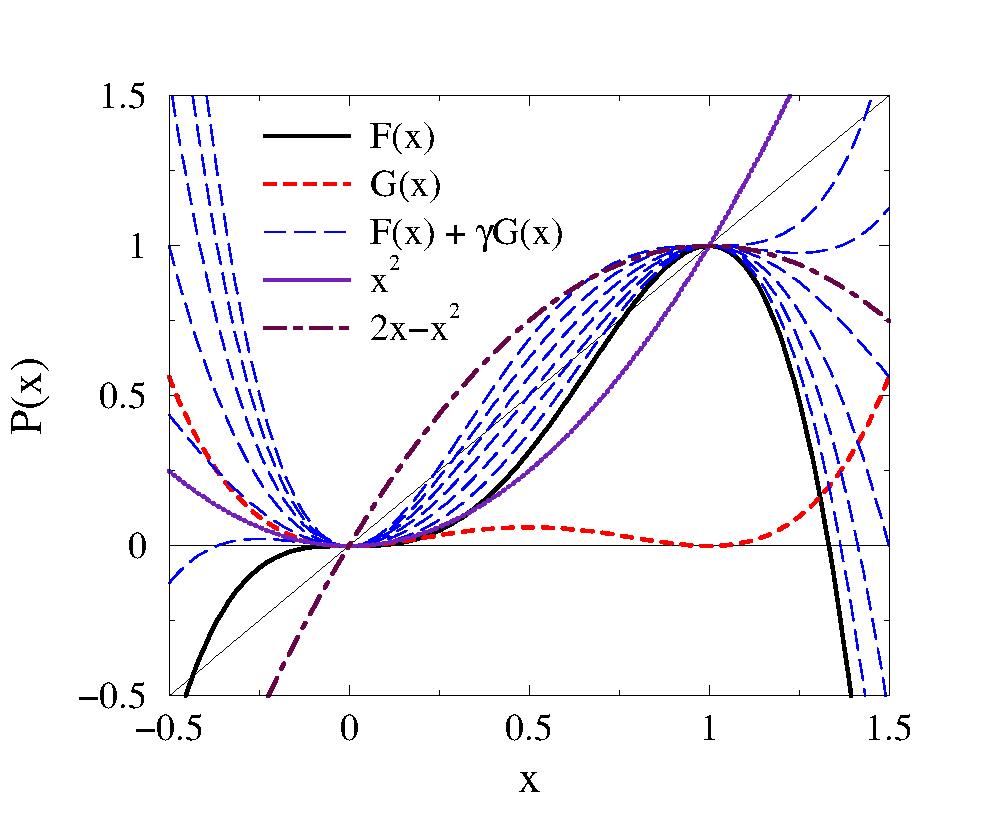
\includegraphics{TP_Fig_F_G_large.eps}
\resizebox*{3.5in}{!}{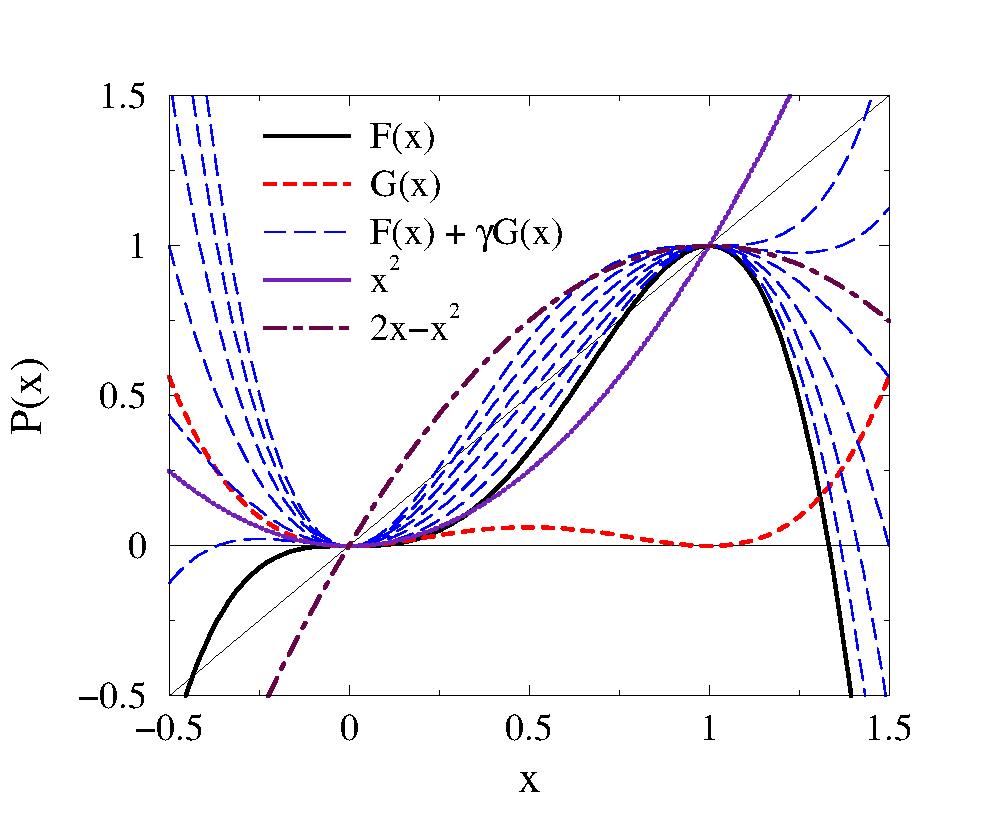
\includegraphics{TP_Fig_F_G_large.eps}}
\end{figure}

Our particular choice of ${\cal F}$ and ${\cal G}$ for the trace setting projection are
\begin{equation} \label{FG}
\left\{ \begin{array}{ll}
{\cal F}(x) &= x^2 (4x-3x^2) \\
{\cal G}(x) &= x^2 (1-x)^2 ,
\end{array} \right.
\end{equation}
which are the depicted functions in Fig. \ref{Fig_F_G}.
The adjustment factor $\gamma$ is bounded such that $\gamma \in [0,6]$.
At convergence $\gamma \rightarrow 3$,
which means that the expansion polynomial ${\cal P}(x) = {\cal F}(x) + \gamma {\cal G}(x)$ 
finally converges to the McWeeny polynomial similar to the PM scheme.
The choice of $\cal F$ and $\cal G$ is quite arbitrary, but this particular
choice has turned out to be both efficient and simple.
The fourth order projection polynomial ${\cal F}(x)$ 
requires only two matrix multiplications, the same as for
the third order McWeeny polynomial, but with one additional
vanishing derivative at $x=0$. Adding the perturbation $\gamma {\cal G}(x)$ with
$\gamma$ increasing from $0$ to $6$ continuously changes the composite 
polynomial ${\cal P}(x) = {\cal F}(x) + \gamma {\cal G}(x)$ to $\cal F$'s mirror 
function $1-{\cal F}(1-x)$ at $\gamma = 6$ with the extra vanishing derivative at $x=1$.
Many other choices of $\cal F$ and $\cal G$ can be made, maybe even more efficient than
what's given in Eq.\ (\ref{FG}). In this way the trace setting
expansion technique can be viewed as a framework for a set
of purification polynomials of varying order.
The algorithm can be described by the following pseudo-code:
\begin{equation} \label{Alg}
\begin{array}{l}
{\it function~ } {\bf P}( {\bf F}, N_e, {\it ErrorLimit})\\
{\it estimate~} \varepsilon_0({\bf F}),~\varepsilon_N({\bf F}) \\
{\bf X}_0 = (\varepsilon_{\rm N}{\bf I}-{\bf F})/(\varepsilon_{\rm N}-\varepsilon_{\rm 0}) \\
{\it while~ Error > ErrorLimit} \\
~~ \gamma_n =(N_e - {\rm Tr} [{\cal F}({\bf X}_n ) ])/{\rm Tr} [{\cal G}({\bf X}_n ) ]\\
~~ {\it if}~ \gamma_n  > \gamma_{\rm max}  \\
~~ ~~ {\bf X}_{n+1} = 2{\bf X}_n-{\bf X}_n^2~~~~~~(i)  \\
~~ {\it else~ if}~ \gamma_n  < \gamma_{\rm min}  \\
~~ ~~ {\bf X}_{n+1} = {\bf X}_n^2~~~~~~~~~(ii) \\
~~ {\it else}\\
~~ ~~ {\bf X}_{n+1} = {\cal F}({\bf X}_n) + \gamma_n  {\cal G}({\bf X}_n)~~~(iii) \\
~~ {\it end}\\
~~ {\it estimate~ Error} \\
{\it endwhile}\\
{\bf P} = {\bf X}_n .
\end{array}
\end{equation}
The estimate of the the spectral bounds of $\bf F$, i.e. 
$\varepsilon_0({\bf F})$ and $\varepsilon_N({\bf F})$ can be given
by, for example, Gersgorin estimates \cite{Palser98}
or via a couple of Lanczos iterations \cite{Daniels99},
with only a small extra computational cost. In the present
article we have chosen the Gersgorin bound, which is
always giving an upper or lower eigenvalue estimate.
It is less accurate than, for example, a Lanczos
estimate. This leads to a somewhat compressed
spectra of ${\bf X}_0$ on $[0,1]$ and a slightly shifted
stepfunction expansion compared to an exact estimate.
This has generally little effect on the TS4 scheme but
could sometimes, at low or high occupancies, make a difference
for the PM scheme, which is more sensitive to the initial
guess.

A main reason for the increased efficiency of TS4 compared to the PM scheme is 
the fact that the derivative at $0$ and $1$ of the spectral projections 
no longer approaches $1$ in the limit of no or maximum
occupancy as in the case of the PM scheme avoiding a spectral
projection that is close to identity, which leads to a slow
convergence in the trace conserving approach. Moreover, it is more efficient to 
work with 4th order polynomials. In this way one extra vanishing
derivative at the fixed points may be achieved, essentially without any
extra computational cost since a 4th order polynomial can be
calculated with only two matrix-matrix multiplications. The
same number of matrix multiplications is needed for a third
order polynomial as in the Mc Weeny or the PM scheme. 
Order 2, 4 and 9 seems to be optimal \cite{Niklasson02}.
An additional important reason is the the slope of the
purification polynomials at the infection point which should
be as steep as possible which favours assymetric purification 
compared to the symmetric cases \cite{Niklasson02b}.


\section{Degeneracy}\label{Degen}

One advantage with the trace setting scheme and the trace
conserving PM scheme, compared to some variational schemes \cite{Li93}
and the grand canonical purification method,
are their ability to deal with degeneracy and fractional occupancy.
Below we briefly discuss the problem with degeneracy and fractional
occupancy, how they destroys idempotency and how they can be calculated
from the density matrix.

Consider the density matrix ${\bf P}$  with a $\nu$ folded degeneracy
with $n_d$ occupied degenerate states. The trace of the density matrix
can be described as
\begin{equation}
Tr [ {\bf P}  ] = N_e = N_e-n_d + \nu \tau,
\end{equation}
where $\tau = n_d/\nu$ is the filling factor of the degenerate states.
In the case of fractional filling of a non-degenerate state at the
chemical potential $\nu = 1$ and $\tau = n_d < 1$.
The density matrix can be described in analogy with Eq. (\ref{Density} as
\begin{equation}\label{Density}
{\bf P} = \sum_{k=1}^{N_{\rm el}-n_d} {\bf c}^{\rm T}_{k} {\bf c}_{k} +
 \sum_{k=N_{\rm el}-n_d +1}^{N_{\rm el}- n_d + \nu } \tau {\bf c}^{\rm T}_{k} {\bf c}_{k}
\end{equation}
and with an orthogonal representation we have that
\begin{equation}
{\bf P}^m = \sum_{k=1}^{N_{\rm el}-n_d} {\bf c}^{\rm T}_{k} {\bf c}_{k} +
 \sum_{k=N_{\rm el}-n_d +1}^{N_{\rm el}- n_d + \nu } \tau^m {\bf c}^{\rm T}_{k} {\bf c}_{k}.
\end{equation}
For powers of the density matrix we thus have that
\begin{equation} \label{Rhom}
{\rm Tr} [ {\bf P}^m  ] = N_{\rm el} - n_d + \nu \tau^m \neq Tr  [ {\bf P} ] = N_{\rm el}.
\end{equation}
From Eq.\ (\ref{Rhom}) we see that idempotency is not
fulfilled (when $m>1$) in the case of degeneracy or fractional filling. 
This means, for example, that grand canonical purification does not work and
that the McWeeny constraint in conjugate gradient
minimization schemes cannot be applied \cite{Li93}.
In order to achieve a constrained search also
in the degenerate case the trace imposing polynomials
${\cal F}({\bf X}) + \gamma {\cal G}({\bf X})$ above, or the trace conserving polynomials
in the canonical PM scheme may possibly be used as alternatives.

Equation (\ref{Rhom}) can be used, as long as
$n \neq \nu$, to calculate the degenerate filling factor and the degeneracy.
Solving the equations (with $m=1,2,3$) for the degeneracy and occupancy
of the degenerate states we get
\begin{equation}
n_d = \frac{({\rm Tr} [{\bf P}-\rho_0^2 ])^2}{{\rm Tr} [{\bf P}-2{\bf P}^2+{\bf P}^3 ]},
\end{equation}
\begin{equation}
\nu = \frac{({\rm Tr} [{\bf P}-{\bf P}^2 ])^3}{{\rm Tr} [{\bf P}^2-{\bf P}^3 ]
{\rm Tr} [{\bf P}-2{\bf P}^2+{\bf P}^3 ]}
\end{equation}
and
\begin{equation}
\tau = \frac{{\rm Tr} [{\bf P}^2-{\bf P}^3 ]}{{\rm Tr} [{\bf P}-{\bf P}^2 ]}.
\end{equation}
These formulas can be viewed as alternative conditions to idempotency
for a degenerate density matrix or in the case of fractional occupancy. 
The relations can also be used
to derive the value of $\gamma_n$ at convergence. For the particular
choice of functions $\cal F$ and $\cal G$ above, Eq.\ (\ref{FG}), we have that
\begin{equation}
\lim_{n \rightarrow \infty} \gamma_n = \frac{n_d - \nu {\cal F}(\tau )}
                                               {\nu {\cal G}(\tau )}.
\end{equation}
Notice, that if $\gamma_{\infty}$
is outside its bounds of stability, i.e.\ if $\gamma_{\infty} \notin [0,6]$, we cannot deal with
degeneracy and fractional filling. The scheme will still
converge, but not to the correct density matrix. For example,
a 100 folded degeneracy requires $n_d \in [24,76]$ otherwise
$\gamma$ will be out of bound at convergence. This puts some
limitations on the ability to treat degeneracy and fractional filling
with the proposed trace setting algorithm.


\section{Thresholding, Error and Stability} \label{Error}

To achieve ${\cal O}(N)$ scaling when solving for the density matrix, sparsity 
must be enforced to prevent fill in following matrix-matrix multiplications.
The most common approach to achieving this sparsity involves an atom-atom or radial cutoff
\cite{XLi93,SQiu94,SItoh95,EHernandez95B,ACanning96}, 
beyond which matrix elements elements are not computed:
\begin{subequations}\label{CutOff}
\begin{eqnarray}
X_{\bf AB}&=&X_{\bf AB} ~~\mbox{\rm iff} ~~|{\bf A -B}| < R_{cut}\\
&=&0 ~~\mbox{\rm else},
\end{eqnarray}
\end{subequations}
allowing all matrices to employ the same graph. This technique has not been used
in the present study. Instead we use a sparse 
atom-blocked linear algebra\cite{Challacombe99,MChallacombe00} (MATT check references!),
 with thresholding at the level of atom-atom blocks:
\begin{subequations}
\begin{eqnarray}
{\bf X}_{AB}&=&{\bf X}_{AB} ~~\mbox{\rm iff} ~~ ||{\bf X}_{AB} ||_F > \tau \\
&=&0 ~~\mbox{\rm else},
\end{eqnarray}
\end{subequations}
where $||\cdot||_F$ is the Frobenious norm. An alternative to blocking 
is to drop element by element\cite{ADaniels97}, which generates maximum sparsity
and is somewhat similar to a change in the computational machine epsilon, i.e. the numerical resolution.  
In either case, we assume a filter opperation is applied after every sparse matrix-matrix 
multiply to avoid fill in,
\begin{eqnarray}
{ \widetilde{ \bf X}}&=&\mbox{\tt Filter} [\bf X,\tau ] \label{filter} \\
	      &=&{\bf X}+\bm{\epsilon},\nonumber 
\end{eqnarray}
leading to the approximate matrix $\widetilde{ \bf X}$ which is in error by $\bm \epsilon$,
a matrix we will asume constant and with $||\bm{\epsilon}|| \sim \tau$ in what follows.

After one matrix-matrix multiply with thresholding we have
\begin{equation}
{\widetilde{ \bf X}}^2 = {\bf X}^2 + \bm{\epsilon}\cdot {\bf X} +{\bf X} 
\cdot \bm{\epsilon}+{\cal O}(\bm{\epsilon}^2).
\end{equation}
Following this thresholding policy, droping second and higher order error terms in $\bm\epsilon$, 
repeated purification iterations leads initially to the behavior
\begin{equation}
{\widetilde{\bf{ X}}}_n  = {\bf X}_n + {\cal O}(  k^n ||\bm{\epsilon}||),
\end{equation}
for some constant $k>1$, depending on the purification scheme.
At first glance this would seem to lead to an unbounded exponential growth of error in purification. 
However, the number of iterations $M$ required by purification schemes to reach convergence has been
shown to scale as \cite{Niklasson02b}
\begin{equation}
\label{Mlog}
M = \alpha + \beta \log_2 \Delta g^{-1},
\end{equation}
where $\Delta g$ is the band gap at the chemical potential, and
the constants $\alpha$ and $\beta$ depend on the projection polynomial, occupancy and accuracy goals.
At worst we thus have an error that is proportional to $||\bm{\epsilon}||$ and inversely
proportional to the band gap $\Delta g$.
Also, as ${\bf X}_n$ enters the regime of quadratic convergence it approaches 
the nearly idempotent matrix $\bf P$.  At this point, the accumulation 
of thresholding errors transitions from exponential to linear growth. 
For example,  $n$-fold iteration of the filtered McWeeny sequence 
close to idempotency leads to the following
fixed point with weak linear drift:
\begin{equation}
{\bf P}={\bf P}+\bm{\epsilon} \cdot {\bf Q}+ (n-1){\bf P}\cdot \bm{\epsilon} \cdot{\bf Q} 
+ {\cal O}(\bm{\epsilon}^2),
\end{equation}
where ${\bf Q}={\bf I}-{\bf P}$ is the virtual projector.
Of course our threshold must be small enough to approach approximate idempotence to achieve
this stabilization. We also see that if no further thersholding is performed
the solution is fix and even the small linear drift dissapears.
Purification is thus numerically stable to initial errors due to thresholding
or finite erithmetics.

Compared to the total accumulated error the idempotency error
at covergence $||{\bf P} - {\bf P}^2||$ is small. The main source of 
error is instead due to the commutation $||\{ {\bf F},{\bf P} \} || $. 
In the exact case $|| \{ {\bf F},{\bf P}_{\rm ex} \} || =0$.
Under numerical thresholding it is the early accumulation of errors preceeding 
convergence that are of special concern, as error accumulation stabilizes at convergence 
increasing only linearly and with a small prefactor goverened by $\tau$.  To address 
this concern we propose the following threshold update
\begin{equation}
\tau_m = \min ( \delta \nu^m,1)*\tau
\end{equation}
where $m$ is purification step.  The parameters $\delta$ and $\nu$ at this point are chosen 
emprically to bring the accumulated error to a level consistent the truncation error, which 
is the error expected purely from truncation of the exact density matrix with $\tau$.
However, even if the exponential thersholding sheme above looks appealing it does not
seem practical or necessary and it has not been used in the present study.


\section{Results}

In order to analyze and demonstrate properties of the quartic trace setting method (TS4)
a comparison is made with the truncated exact density-matrix solution (TES), and the 
Palser-Manolopoulos scheme (PM) \cite{Palser98} implemented in an {\it ab initio}
linear scaling total energy scheme for electronic structure calculations.
Atomic units are used throughout. 

\subsection{Implementation}

\subsubsection{Programming}
The algorithms were implemented in the {\sc MondoSCF}v1.0a4 suite of 
quantum chemistry programs\cite{MondoSCF}.  
All sparse matrix computations employ the same blocked compressed sparse row 
(BCSR)\cite{Challacombe99,MChallacombe00} {MATT check references!) 
data structure.  With the BCSR data structure, the cost of recomputing the symbolic 
matrix is negligible, allowing dynamic fill-in.  Also, the BCSR matrix-matrix multiplies 
are carried out in highly optimized C for small 
(5x5x5 to 15x15x15) dense matrix-matrix multiplies. 

The code was compiled using the 
Portland Group F90 compiler {\sc pgf90}v3.2 \cite{pgf90} with the {\tt -O1 -tp athlon} 
options  and with the gnu C compiler {\sc gcc}v2.96 using the {\tt -O1} flag.  All 
calculations were carried out on a 1.2GHz AMD Athlon Thunderbird running RedHat 
{\sc Linux}v7.3\cite{RedHat73} (MATT check references!).  The exact eigensolution was carried out with the native
{\sc LAPACK} \cite{LAPACK}  (MATT check references!) {\sc DSYEV} and {\sc BLAS} supplied with the {\sc pgf90}v3.2 compiler.

All TES calculations employed L{\"o}wdin symmetric orthogonalization \cite{PLowdin50} (MATT check reference!), 
while all TS4 and PM calculations used the congruence transformation provided by
compuation of the sparse approximate inverse AINV \cite{AINV,MChallacombe02c} 
(MATT check references! AINV should be included!) Cholesky factor, except for chlorophyll.

subsubsection{Thresholds and convergence}
Experiments were carried out with the thresholding in the algorithm of Eq. (\ref{Alg})
as follows:
\begin{equation} 
\begin{array}{lll}
i)    &{\bf X}_{n+1} &= {\tt Filter}[2{\bf X}_n - \widetilde{\bf X}^2_n,\tau] \\
ii)   &{\bf X}_{n+1} &= {\tt Filter}[\widetilde{\bf X}^2_n,\tau] \\
iii)  &{\bf Y}_{\rm tmp}     &= {\tt Filter}[\gamma_n + (4-2\gamma_n){\bf X}_n + (\gamma_n-3)\widetilde{\bf X}^2_n,\tau] \\
      &{\bf X}_{n+1} &= {\tt Filter}[\widetilde{\bf X}^2_n {\bf Y}_{\rm tmp},\tau].
\end{array}
\end{equation}
Unless otherwise stated, all errors in the TES coorespond to a single
truncation of the exact solution of the density matrix (to machine precision) with $\tau=10^{-6}$.
No variable thresholding or incremental Fock builds were used in the experiments. 
All calculations also employed DIIS extrapolation \cite{PPulay88}, with the SCF
converged to within $\delta E < 10^{-9}$ and $\Delta{\bf P} < 10^{-5}$ when possible.
Due to thresholding SCF convergence can never be reached exactely.
An SCF termination policy that recognizes this is therefore important,
especially at large thresholds. 

%Conditions for convergence (MATT this is not clear!) of the PM and TS4 algorithms include a rise in relative 
%error of the electronic energy $\delta E_{\rm el}$, a rise in the maximum absolute 
%error in a density matrix element $\Delta{\bf P}$, or meeting the criteria 
%$\delta E_{\rm el} < 10^{-11}$ and $\Delta{\bf P} < 10^{-6}$.  
%All calculations also employed DIIS extrapolation \cite{PPulay88}, with the SCF
%converged to within $\delta E < 10^{-9}$ and $\Delta{\bf P} < 10^{-5}$ when possible.
%Due to thresholding SCF convergence can never be reached exactely.
%An SCF termination policy that recognizes this is therefore important,
%especially at large thresholds. 

%scheme DIIS attempts to extrapolate the between
%cycle, {\em inter-SCF} commutator ($[{\bf F}^{I},{\bf P}^{I-1}]$) to zero.  
%With thresholding however, the {\em intra-SCF} commutator 
%will never be truely zero, and for large accumulation errors this can lead to 
%stagnation of the DIIS.  An SCF termination policy that recognizes this is 
%therefore important.  In {\sc MondoSCF}, there are two additional conditions 
%in addition to the set accuracy goals.  The first looks for a simultaneous increase 
%in both the leading DIIS error vector and the difference density matrix error:
%$\varepsilon^{I+1}_{\rm DIIS}>\varepsilon^{I}_{\rm DIIS}$ and 
%$\Delta {\bf P}^{I+1}> \Delta {\bf P}^{I}$, where 
%$\varepsilon^{I}=||[{\bf F}^{I},{\bf P}^{I-1}]||_F$ and 
%$\Delta {\bf P}^{I}=\max_{P_{ij}}|{\bf P}^I-{\bf P}^{I-1}|$.  The second
%condition detects a stall in convergence corresponding to a relative change in the 
%DIIS error between SCF cycles $\delta { \varepsilon}_{\rm DIIS}<0.09$ and a 
%relative change in the difference density matrix $\delta \Delta {\bf P}<10^{-2}$.  
%For the tight thresholds employed here, these auxiliary conditions are typically
%accessed only for $\tau>10^{-3}$.

\subsection{Water}

\begin{figure}[t]
\resizebox*{3.5in}{!}{\includegraphics{WATER_FIGS/WaterDensityConvergence.eps}}
\caption{Convergence of the TS4 and PM  (H$_2$O)$_{150}$ RHF/6-31G** 
density matrix to idempotence, as measured by the maximum matrix element in 
$|{\bf X}_{N+1}-{\bf X}_N|$. Cycles were continued after convergence.}\label{waterconvergence}
\end{figure}

\begin{figure}[t]
\resizebox*{3.5in}{!}{\includegraphics{WATER_FIGS/WaterFillIn.eps}}
\caption{Fill in of the TS4 and PM density matrices with iteration
for (H$_2$O)$_{150}$ RHF/6-31G**.} \label{fillin}
\end{figure}

%\begin{figure}[t]
%\resizebox*{3.5in}{!}{\includegraphics{WATER_FIGS/EffectsOfBounds.eps}}
%\caption{for (H$_2$O)$_{150}$ RHF/6-31G**.} \label{EigenBounds}
%\end{figure}

A sequence of water clusters (H$_2$O)$_{10}$ through (H$_2$O)$_{150}$  \cite{WaterCluster}
were used to explore the differences between PM, TS4 and ES at the RHF/6-31G** level of theory.  
%This level of theory leads to a large gap, $\Delta g \approx 0.5$, and should easily lead to linear scaling.  
The 6-31G** basis set is large enough to bring out the differences between PM and TS4 
($f_{\rm occ}=0.2$), but not so large as to be impractical in linear scaling calculations.  

In Figure~\ref{waterconvergence}, convergence to idempotence is shown for 
construction of the  RHF/6-31G** (H$_2$O)$_{150}$ density matrix using the PM and TS4 methods
and their local thresholds $\tau=10^{-3}, 10^{-4}, 10^{-5}$ and $10^{-6}$ (indicated
in the paranthesis). Convergence
of TS4 occurs in approximately 18 iterations, and for PM in about 30.  At first, 
one might conclude that the longer iteration count for PM translates into significantly 
longer CPU times reltative to TS4. However, the fill in of the two methods
can be quite different as shown in Figure~\ref{fillin};  the PM method involves much
sparser intermediate matrices than does TS4, which fills in quickly.  The actual ratio
of PM to TS4 CPU times is only about 1.2 with $\tau=10^{-4}$ as shown in 
Figure \ref{cputimes}. At this level of approximation, both methods achieve 
an early onset of true linear scaling, crossing  over the ES time at about 50 water 
molecules. 
%One reason for this early crossover is the aforementioned use 
%{\sc DGEMM}s optimized for small matrices, with which the programs {\sc TS4} and {\sc PM} achieve 
%sustained rates better than 400 Mflop/s. This compares favorably with the dense $n=100$
%{\sc LINPACK} at 558 Mflop/s on this platform \cite{JDongarra01}.

\begin{figure}[b]
\resizebox*{3.5in}{!}{\includegraphics{WATER_FIGS/WaterTimings.eps}}
\caption{CPU time for one SCF cycle of the ES, and 
	 $\tau=10^{-4}$ TS4 and PM with number of water molecules.}\label{cputimes}
\end{figure}

\begin{figure}[b]
\resizebox*{3.5in}{!}{\includegraphics{WATER_FIGS/TS4vsPMWaterCommutatorErrors.eps}}
\caption{The accumulated PM and TS4 commutator errors $||[{\bf F ,P }]||_F$ 
with iteration and the truncation errors corresponding to eigensolution followed
by one filter opperation (straight lines), for tightly converged RHF/6-31G** (H$_2$O)$_{150}$ density 
and Fock matrices.}\label{commerrors}
\end{figure}

\begin{figure}[b]
\resizebox*{3.5in}{!}{\includegraphics{WATER_FIGS/ConvergedWaterErrors.eps}}
\caption{Energy per water molecule with increasing cluster size for TS4 and PM 
         using $\tau=10^{-4}$, and by ES.}\label{waterenergyerrors}
\end{figure}

While the compensation between convergence and fill rates lead to similar CPU times, 
the differences in accumulated errors are quite differenet for the two purification schemes.
This is shown in Figure~\ref{commerrors}, which compares the commutator errors $||[{\bf FP,PF}]||_F$
for PM and TS4 with iteration at $\tau=10^{-3}, \tau=10^{-4}, \tau=10^{-5}$ and $\tau=10^{-6}$
for (included in the parenthesis) RHF/6-31G** (H$_2$O)$_{150}$. 
The commutator errors are a sensitive measure of eigenbasis
blurring due to thresholding.  Also shown in Figure~\ref{commerrors} 
are the truncation errors for these matrix thresholds, corresponding to the TES 
given from the exact density matrix followed by a single threshold with
$\tau = 10 ^{-3}$, $\tau = 10 ^{-4}$, $\tau = 10 ^{-5}$, and $\tau = 10 ^{-6}$.  
In each case, the TS4 accumulated errors are approximately one order of 
magnitude larger than those due to truncation, while the PM accumulated errors are two
orders larger.  Note the decade by decade control of the commutator error by the matrix
threshold, an initial exponential increase in the accumulated error and the 
small linear rise in error upon convergence of the purification schemes as discussed
in Section~\ref{Error}.

%While we have the bound Eq.~\ref{DensCommBound} relating $||[{\bf P}_{\rm ex},{\bf P}]||_2$ 
%to error in the density matrix, the more readily accesible measure $||[{\bf F},{\bf P}]||_F$
%requires  system dependent callibration for use in estimating the error in computed
%properties.  In particular, the eigenvalue spectrum of $\bf F$ will be different from
%system to system; errors in the density matrix will propagate through the one-electron potential
%every SCF cycle, and will have a different impact on convergence depending on sensitivity 
%of the problem to perturbation.  

In Figure~\ref{waterenergyerrors}, 
converged total energies per water molecule are shown for TES, and for PM and TS4 at
$\tau=10^{-4}$.  After an initial broadening, the error per water molecule 
holds constant with system size.  For this system and at this level of 
approximation the order of magnitude difference between PM and TS4 commutator errors 
corresponds to one order of magnitude in the total energy.  

\subsection{C60}

\begin{figure}[h]
\resizebox*{3.5in}{!}{\includegraphics{FULL_FIGS/ConvergedC60Errors.eps}}
\caption{Behavior of the converged PM and TS4 total energies with matrix threshold $\tau$
         for RPBE/STO-6G C60.  The log-log inset shows 
         convergence of the signed absolute error $\Delta E$ for small 
         thresholds and the line $10^{4.4} \tau^2$.}\label{c60convergence}
\end{figure}

%\begin{figure}[h]
%\resizebox*{3.5in}{!}{\includegraphics{FULL_FIGS/C60SCFcycles.eps}}
%\caption{Number of SCF cycles to reach a tight convergence with PM and TS4         
%         for RPBE/STO-6G C60 at the RPBE level of theory.}\label{c60SCFs}
%\end{figure}


In reference~\onlinecite{JDaniels98} (MATT Check reference!), Daniels and Scuseria found the PM method to be 
unstable for semi-empirical calculations on C60 requiring  $\approx 100$ SCF
cycles, and converging to an excited state solution without level shifting.  
We sumarise that this is a result of DIIS pollution 
by large commutator errors due to the use of ``fixed-form'' 
linear algebra (as opposed to dynamic fill-in) and/or the low filling 
$f_{\rm occ} \gtrsim 0.8$ inherent in the semi-empirical approximation, rather
than an intrinsic problem with purification schemes applied to C60.   
It is important therefore to establish reasonable behavior of purification schemes 
for this case,  although  C60 is small with a gap $\Delta g\approx 0.07$ and a
density matrix that should completely fill-in for all but the most dire thresholds. 

As {\sc MondoSCF} does not feature semi-empirical methods, the behavior of PM and TS4 
is instead examined for the smallest possible basis set; STO-6G for which the 
C60 filling factor is $f_{\rm occ}=0.62$. All calculations start with the same spherically 
averaged, block diagonal $1s^22s^22p^2$ guess. The PM and TS4 total 
energies with matrix threshold $\tau \in [10^{-2},10^{-5}]$ are shown in 
Figure~\ref{c60convergence}.  The inset contains the signed absolute errors 
$\Delta E$ relative to the total energy $E_{\rm TES}=-2278.116~453$ and the fit 
$10^{4.4} \tau^2$, demonstrating quadratic convergence. 
While the precise number of matrix-matrix multiplies depends on $\tau$,
$M_{\rm PM}/M_{\rm TS4} \approx 1.2$ and $M_{\rm TS4}=38$ for $\tau=10^{-5}$.

Because tight numerical and convergence thresholds are used throughout, 
except those that depend on the matrix threshold $\tau$ local to {\sc PM} and {\sc TS4},
the number of SCF cycles behaves erratically for large thresholds due to large intra-SCF 
commutator errors that pollute the DIIS SCF solution.  
%This behavior is shown in 
%Figure~\ref{c60SCFs}. For smaller thresholds and TS4, the number of SCF cycles 
%approaches the TES value of 7.  

\subsection{Chlorophyll}

%\begin{figure}[h]
%\resizebox*{3.5in}{!}{\includegraphics{ChIsoRho.jpg}}
%\caption{The electrostatic potential color mapped onto the Chlorophyll electron density isosurface,
%         computed at the RPBE/6-311G(3d,3p) level of theory.  Blue corresponds to a negative potential, 
%         and red is positive.  The iso-density was taken at 0.03 au.}\label{ChPic}
%\end{figure}

\begin{table}
\caption{Dependence of the number of matrix-matrix multiplies $M$, order of the signed absolute 
error in the converged total energy $\Delta E$ for both the PM and the TS4 method with basis set 
progression for RPBE Cholophyll. THe threshold was set to $\tau = 10^{-6}$}
\label{ChlorophyllConvergence}
\squeezetable
\begin{tabular}{lcccccc}
\toprule
Basis set       &  $f_{\rm occ}$ & $E_{\rm RH}$       &$M_{\rm PM}$&$M_{\rm TS4}$& $\Delta E_{\rm PM}$ & $\Delta E_{\rm TS4}$ \\
\colrule
STO-3G          &  0.62      & -2348.268  & 63      & 45       & $ 10^{-6}$   &  $ 10^{-7}$   \\ 
3-21G           &  0.34	     & -2365.182  & 59      & 47       & $ 10^{-6}$   &  $ 10^{-8}$   \\
Ahlrichs VDZ    &  0.34      & -2375.971  & 59      & 43       & $ 10^{-7}$   &  $ 10^{-8}$   \\
6-31G**         &  0.19      & -2378.313  & 75      & 48       & $ 10^{-6}$   &  $ 10^{-7}$   \\
Ahlrichs VTZ    &  0.21      & -2378.400  & 107     & 57       & $ 10^{-3}$   &  $ 10^{-7}$   \\
6-311G**        &  0.15      & -2378.853  & 115     & 55       & $ 10^{-4}$   &  $ 10^{-7}$   \\
%6-311G(2d,2p)   &  0.11      & -2378.930  & 147     & 61       & $ 10^{-3}$   &  $ 10^{-8}$   \\
%6-311G(3d,3p)   &            & -2378.970  &         &          &              &        \\
\botrule
\end{tabular}
\end{table}

Linear scaling methods in the large basis set limit have heretofore been largely
ignored.  However, as parallel ${\cal O}(N)$ methods mature it is likely that  this 
regime will be accessed more frequently.

Here, TES, PM and TS4 are used in the basis set progression 
of Chlorophyll, a relatively small (91 atom) Mg containing porhyrin ring system. 
Symmetric L\"owdin orthogonalization was used siince it is less sensitive
to the high condition numbers arising from the extended basis sets.
%The electrostatic mapped electron density isosurface of Chlorophyll at the
%RPBE/6-311G(3d,3p) level of theory is shown in Figure~\ref{ChPic}. 
In Table~\ref{ChlorophyllConvergence}, total energies computed with TES, the number 
of matrix-matrix multiplies and the absolute signed error in the total energies are 
presented.  Although the Fock-derived initial guess for the PE methods is initially 
close to $99\%$ dense, PM takes a more sparse path towards convergence, 
droping to $\approx 90\%$ full as in Figure~\ref{fillin}.  Also, as the basis set 
size increases so does the number of matrix-matrix multiplies $M_{\rm PM}$ required 
for PM to reach convergence. For the larger basis sets the behavior of PM becomes 
pathological,  leading to errors greater than a $m$hartree even with quite a tight
threshold ($\tau=10^{-6}$).  On the other hand, the TS4 accumulated error remains
stable at about 0.1 $\mu$hartree.

\section{Discussion}

A recent WTEC workshop on computational chemistry \cite{WTEC00} (MATT Check reference!) noted that when it comes
to linear scaling ``the devils are in the details''. These details include
interplay between the interative density matrix solver, the underlying incomplete sparse 
linear algebra, basis set approximations and methods for convergence acceleration.   
Despite these complexities, TS4 is a clear improvment relative to PM, arguably the best 
PE approach to date.  
In particular,  for RHF/6-31G** water clusters accumulated errors in the TS4 total energy 
were shown to be an order of magnitude smaller than PM with $\tau=10^{-4}$.  
For larger basis sets, PM was shown to behave pathologically even 
for a small system and with tight numerical thresholds, while TS4 was able to maintain
sub-$\mu$hartree accuracy.  This pathology stems from domination of the eigenspectrum
by the virtual space, skewing the PM polynomial to form a step close to $0$
where it looses efficiency since the polynomials initially become close
to identity. Improving on the starting guess, using the
exact spectral bounds instead of the Gersgorin estimate, as used in the present study, 
may partly shift the occupation limit where the PM scheme gives large errors, however the
basic deficiency still remains. Having relaxed the trace-preserving constraint, TS4
does not suffer this problem.
%One approach to avoiding these difficulties might be to employ 
%{\em in situ} basis set optimization \cite{Conquest,JTalman00,GBerghold02}, allowing 
%high accuracy with a reduced representation.
At the same time it is still possible to deal with degeneracy and fractional occupancy.

Under thresholding intra-SCF errors corrupt DIIS, preventing 
extrapolation of the inter-SCF commutator to zero.  For thresholds $\tau \lesssim 10^{-4}$
this is not a problem, and for larger thresholds other convergence 
accelerators may be more stable under perturbation.  Nevertheless,
the use of auxilliary SCF convergence criteria 
to detect DIIS stagnation does allow robust application of PE methods
under severe thresholding ($\tau \approx 10^{-2})$.
In particular, no intrinsic problems (excited states, non-convergence, etc) were
found in application to RPBE/STO-6G C60, although extra SCF cycles were sometimes required. 
In all cases the approximate PE total energies were found to approach the TES values
from above, and for C60 were shown to converge quadratically with $\tau$.
Clearly the effect of both accumulated and truncation errors is to move 
$[\bf P,F]$ away from zero.  Of special concern is smoothness
of the energy surface subject to these errors \cite{DBowler00} (MATT check reference! Bowler99?).  As pointed out by 
Bowler \cite{DBowler00} (MATT check reference! Bowler99?),  the accumulation errors can be reduced 
(at least to the level of truncation) by following PE with DMM. 
It is also possible to achieve the same effect with PE only, but with a tighter matrix threshold.  
Here again there may be differences between numerical thresholds and radial cutoffs 
that are not yet fully appreciated. It is certain though that the faster convergence of TS4 can 
lead to faster CPU times in the small and large basis set limit with the static graphs 
that are obtained using radial cut-offs. Note, that even if TS4 and the PM scheme are 
non-variational formulation of the single particle density matrix, the self-consistent
total energy formulation is still variational. Thresholding limits the variational space
both in the constrained DMM schemes and the PE methods, generally giving rise to a slightly
higher total energy compared to exact arithmetics.

\section{Conclusions}

In summary we have proposed a general, simple, and efficient 
trace setting density-matrix expansion algorithm that converges 
to the correct occupation without prior knowledge of the chemical
potential. The scheme was shown to compare favorably with the
similar canonical trace conserving PM method, especially at
low and high occupancies. The methods ability to give the
correct expansion also for degenerate systems or for problems
with a fractional occupancy was discussed
and formulas for calculating the degeneracy and filling factors
from the density matrix were derived. 
The numerical stability in the case of thresholding
was discussed and analyzed. The method was implemented in
MONDOSCF suite of {\it ab initio} linear scaling electronic structure
programs and compared to the PM scheme and the
truncated exact solution and the numerical stability
and error was analyzed.

total accumulated error of the converged density matrix is independent
of the number of matrix multiplications. The main error 
is instead due to the size of the inverse band gap which, however,
may lead to problems for large metallic systems.

\section{Acknowledgement}


\bibliographystyle{apsrmp}
\bibliography{mondo}


\begin{references}

\bibitem{Corr} Anders M.\ N.\ Niklasson email: niklasson@lanl.gov.

\bibitem{Goedecker_RMP_99} S. Goedecker,
Rev.\ Mod.\ Phys. {\bf 71}, 1085 (1999).

\bibitem{Hohenberg64} P. Hohenberg and W. Kohn,
Phys.\ Rev.\ {\bf 136}, B864 (1964).

\bibitem{Kohn65} W. Kohn and L.J. Sham,
Phys.\ Rev.\ {\bf A1133} (1965).

\bibitem{Sameh82}  A.\ H. Sameh and J.\ A. Wisniewski,
SIAM Journal on Numerical Analysis {\bf 19}, 1243 (1982).

\bibitem{Li93} X.\ -P. Li, W. Nunes, and D. Vanderbilt,
Phys.\ Rev.\ B {\bf 47}, 10891 (1993).

\bibitem{Carlsson95} A. E. Carlsson,
Phys.\ Rev.\ B {\bf 51}, 13 935 (1995).

\bibitem{Hernandez96} E. Hernandez, M.\ J. Gillan, and C.\ M. Goringe,
Phys.\ Rev.\ B {\bf 53}, 7147 (1996).

\bibitem{Kohn96} W. Kohn,
Phys.\ Rev.\ Lett. {\bf 76}, 3168 (1996).

\bibitem{Daniels97} A.\ D. Daniels, J.\ M. Millam, and G.\ E.\ Scuseria,
J.\ Chem.\ Phys. {\bf 107}, 425 (1997).

\bibitem{Yang97} W. Yang,
Phys.\ Rev.\ B {\bf 56}, 9294 (1997).

\bibitem{Stephan98} U. Stephan, and D.\ A. Drabold,
Phys.\ Rev.\ B {\bf 57}, 6391 (1998).

\bibitem{Challacombe99} M. Challacombe,
J.\ Chem.\ Phys. {\bf 110}, 2332 (1999).

\bibitem{Haynes99} P.\ D. Haynes, and M.\ C. Payne,
Phys.\ Rev.\ B {\bf 59}, 12 173 (1999).

\bibitem{Bowler99} D.\ R. Bowler and M.\ J. Gillan,
Comp.\ Phys.\ Comm. {\bf 120}, 95 (1999).

\bibitem{Daniels99} A.\ D. Daniels and G.\ E.\ Scuseria,
J.\ Chem.\ Phys. {\bf 110}, 1321 (1999).

\bibitem{McWeeny60} R. McWeeny,
Rev.\ Mod.\ Phys. {\bf 32}, 335 (1960).

\bibitem{Goedecker94} S. Goedecker and L. Colombo,
Phys.\ Rev.\ Lett. {\bf 73}, 122 (1994).

\bibitem{Palser98} A.\ H.\ R. Palser and D.\ E. Manolopoulos,
Phys.\ Rev.\ B {\bf 58}, 12704 (1998). 

\bibitem{Beylkin99} G. Beylkin, N. Coult, and M.\ J. Mohlenkamp,
J.\ Comp.\ Phys. {\bf 152}, 32 (1999).

\bibitem{Holas01} A. Holas, Chem.\ Phys.\ Lett.\ {\bf 340}, 552 (2001).

\bibitem{Niklasson02} A.\ M.\ N. Niklasson, C.\ J. Tymczak, and H. R\"oder,
{\it "A multi-resolution density matrix approach to electronic structure
calculations"} (Accepted to PRB).

\bibitem{Niklasson02b} A.\ M.\ N. Niklasson, {\it Expansion
algorithm for the density matrix}, (Accepted to PRB).

\bibitem{Kenney95} C.\ S. Kenney, and A.\ J. Laub,
IEEE Trans. Automat. Control {\bf 40}, 1330 (1995).

\bibitem{Kohn59} W. Kohn,
Phys.\ Rev.\ {\bf 115}, 809 (1959).

\bibitem{Baer97} R. Baer and M. Head-Gordon,
Phys.\ Rev.\ Lett. {\bf 79}, 3962 (1994).

\bibitem{Stephan00} U. Stephan, R.\ M. Martin, and D.\ A. Drabold,
Phys.\ Rev.\ B {\bf 62}, 6885 (2000)

\bibitem{Beylkin91} G. Beylkin, R. Coifman, and V. Rokhlin,
Commun.\ Pure Appl.\ Math. {\bf 44}, 141 (1991).

\bibitem{Goedecker99} S. Goedecker and O.\ V. Ivanov,
Phys.\ Rev.\ B {\bf 59}, 7270 (1999).

\bibitem{White92} S.\ R. White,
Phys.\ Rev.\ Lett. {\bf 69}, 19 2863 (1992).

\bibitem{Nemeth00} K.\ Nemeth, and G.\ E.\ Scuseria,
Journal of Chemical Physics. {\bf 113}, 6035 (2000).

\bibitem{Denman81} E.\ D. Denman, and J. Leyvaramos,
Applied Math. Comp. {\bf 8}, 237 (1981).

\bibitem{Howland83} J.\ L. Howland,
Linear algebra and its applications {\bf 49}, 221 (1983).~

\bibitem{Mondo} M. Challacombe and E. Schwengler,
J.\ Chem.\ Phys. {\bf 106}, 5526 (1997).
E. Schwengler, M. Challacombe and M. HeadGordon,
J.\ Chem.\ Phys. {\bf 106}, 9708 (1997).
M. Challacombe, J.\ Chem.\ Phys. {\bf 110}, 2332 (1999).
M.  Challacombe, J.\ Chem.\ Phys. {\bf 113}, 10037 (2000).

\bibitem{WaterCluster} Can be downloaded from  http://www.t12.lanl.gov/~mchalla


\end{references}

\end{document}
